\documentclass{beamer}
\usepackage[utf8]{inputenc}
\usepackage{polski}
\usepackage[polish]{babel}
\usepackage[T1]{fontenc}
\usepackage{multicol}
\usepackage{amsmath}
\usepackage{mathtools}

\mode<presentation>
{
  \usetheme{Madrid}
  \usecolortheme{beaver}
  \usefonttheme{default}
  \setbeamertemplate{navigation symbols}{}
  \setbeamertemplate{caption}[numbered]
} 


\usepackage{graphicx}
\DeclareGraphicsExtensions{.png,.jpg}

\title[Elasticsearch]{Elasticsearch}
\author{Jakub Podeszwik}
\institute{Yameo}
\date{28.03.2019}

\AtBeginSection[]{
	\begin{frame}
		\begin{center}
			\usebeamerfont{section title}\Large\insertsection
		\end{center}
	\end{frame}
}

\begin{document}

\begin{frame}
  \titlepage
\end{frame}

\begin{frame}{Apache Lucene}
	\begin{enumerate}
		\item Full text search library written in Java
		\item initlally released in 1999
		\item in 2010 Apache Solr joined Lucene as subproject
	\end{enumerate}
\end{frame}
\begin{frame}{Elasticsearch}
	\begin{enumerate}
		\item Open source Full text search Engine writen on top of lucene
		\item 02.2010 - version 0.4 released
		\item 02.2014 - version 1.0 released
		\item scalable, near realtime, highly available, restful
	\end{enumerate}
\end{frame}
\begin{frame}{Inverted index}
	\begin{figure}
		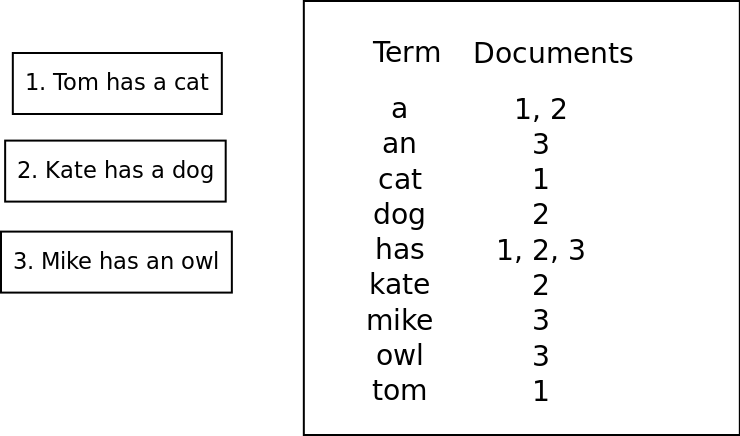
\includegraphics[width=\textwidth,height=7cm,keepaspectratio=true]{inverted-index}
	\end{figure}
\end{frame}

\begin{frame}{Lucene Segment}
	Immutable, stored on disk data structure consisting of:
	\begin{enumerate}
		\item inverted index
		\item fielddata cache / doc\_values
		\item \_source
		\item live documents bitset (this one is not immutable)
		\item ...
	\end{enumerate}
\end{frame}

\begin{frame}{Lucene index}
	\begin{figure}
		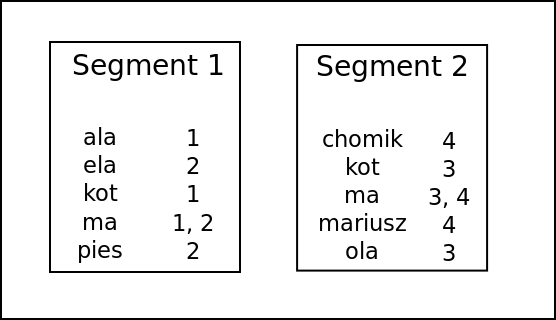
\includegraphics[width=\textwidth,height=7cm,keepaspectratio=true]{lucene-index}
	\end{figure}
\end{frame}
\begin{frame}{Segments merging}
	\begin{figure}
		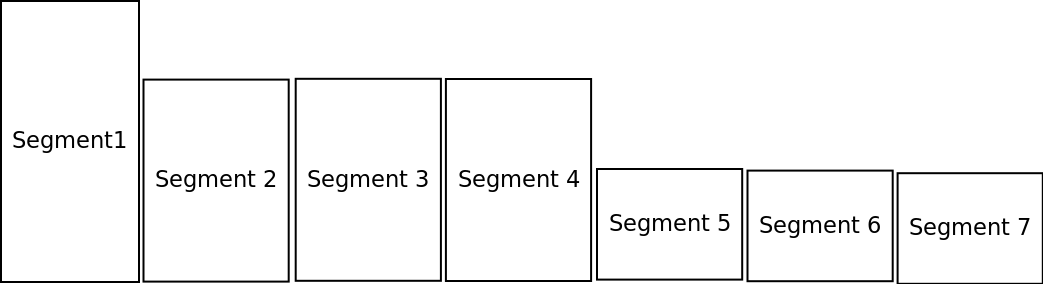
\includegraphics[width=\textwidth,height=7cm,keepaspectratio=true]{segments}
	\end{figure}
\end{frame}
\begin{frame}{Segments merging}
	\begin{figure}
		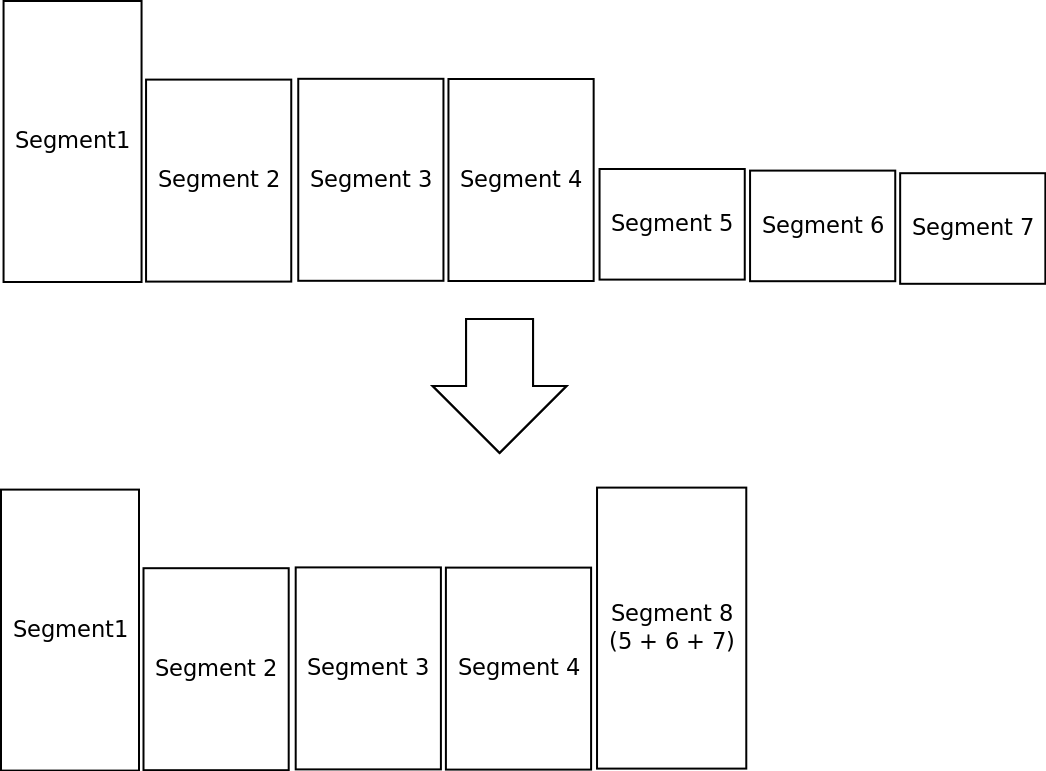
\includegraphics[width=\textwidth,height=7cm,keepaspectratio=true]{segments-merging}
	\end{figure}
\end{frame}
\begin{frame}{Elasticsearch index}
	\begin{figure}
		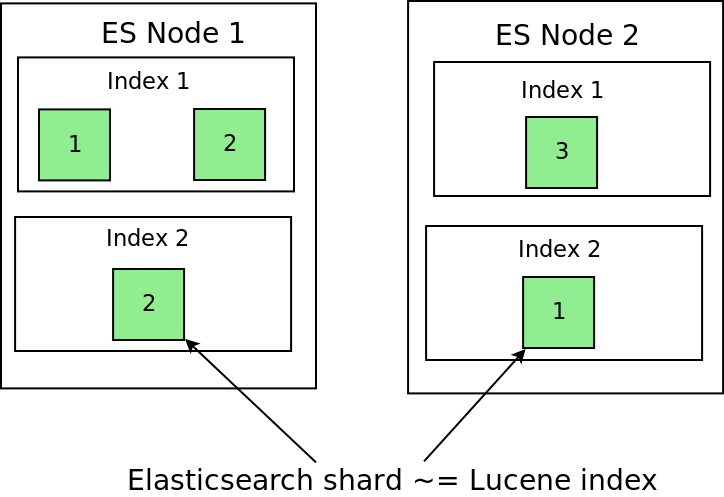
\includegraphics[width=\textwidth,height=7cm,keepaspectratio=true]{elasticsearch-index}
	\end{figure}
\end{frame}
\begin{frame}{Elasticsearch index}
	\begin{figure}
		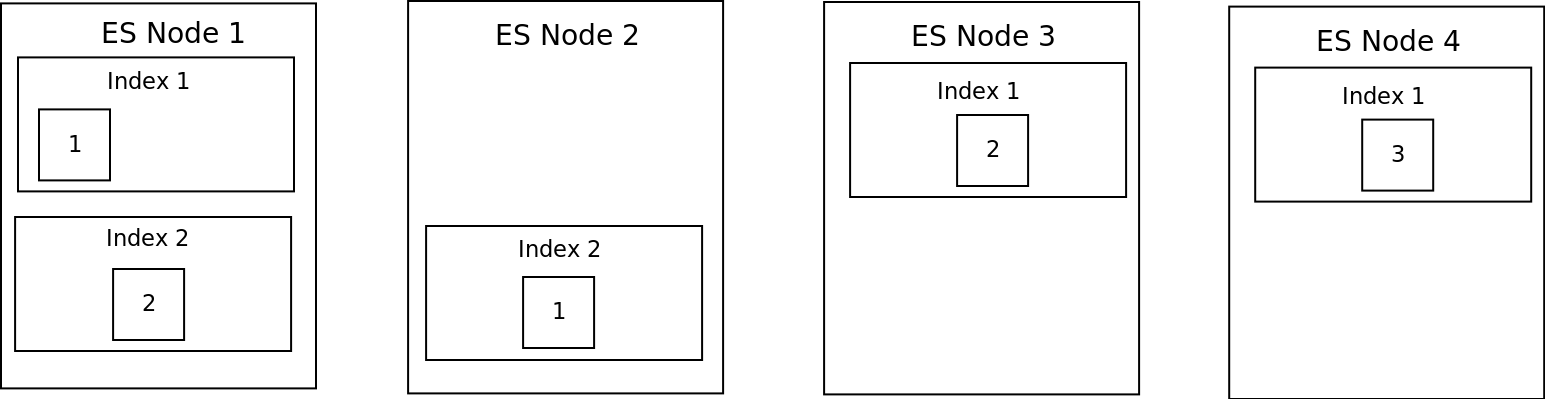
\includegraphics[width=\textwidth,height=7cm,keepaspectratio=true]{elasticsearch-more-nodes}
	\end{figure}
\end{frame}
\begin{frame}{Elasticsearch shard replicas}
	\begin{figure}
		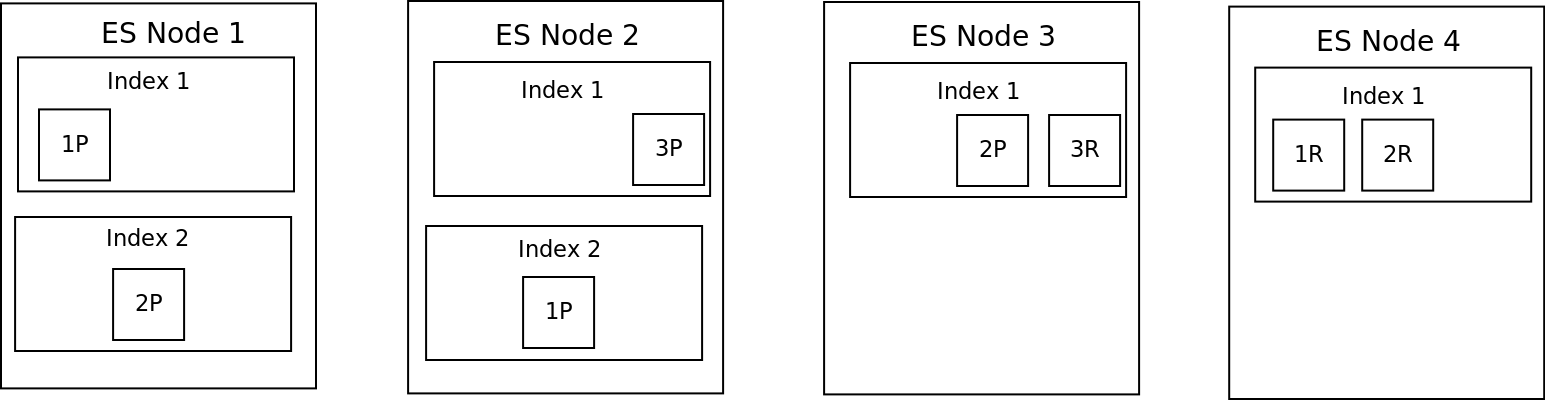
\includegraphics[width=\textwidth,height=7cm,keepaspectratio=true]{elasticsearch-shard-replicas}
	\end{figure}
\end{frame}
\begin{frame}{Translog}
	\begin{figure}
		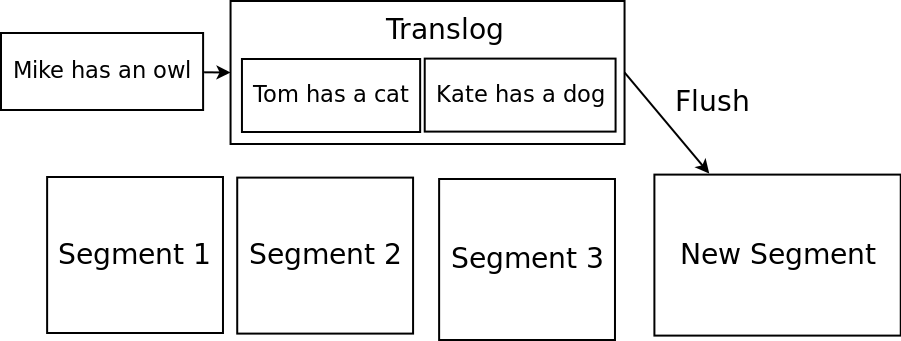
\includegraphics[width=\textwidth,height=7cm,keepaspectratio=true]{translog}
	\end{figure}
\end{frame}
\begin{frame}{Search}
	\begin{figure}
		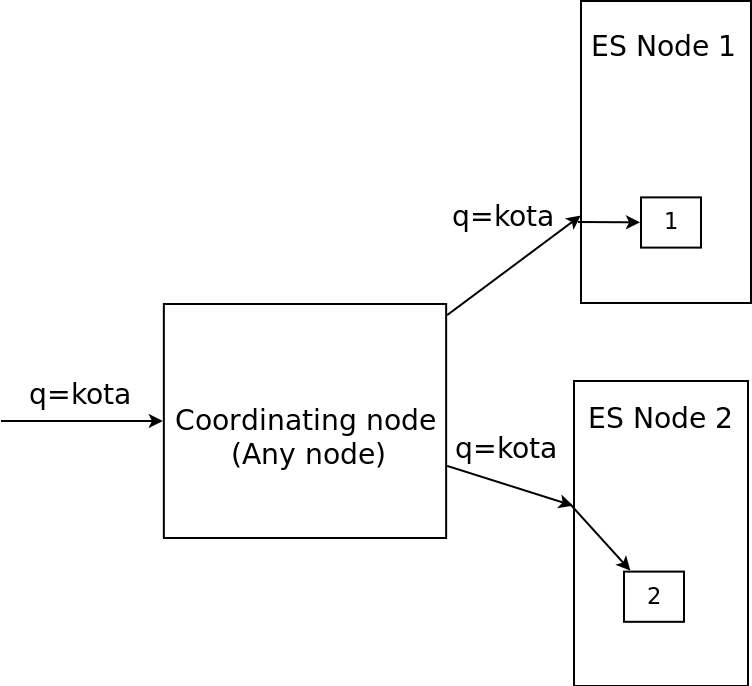
\includegraphics[width=\textwidth,height=7cm,keepaspectratio=true]{search1}
	\end{figure}
\end{frame}
\begin{frame}{Search}
	\begin{figure}
		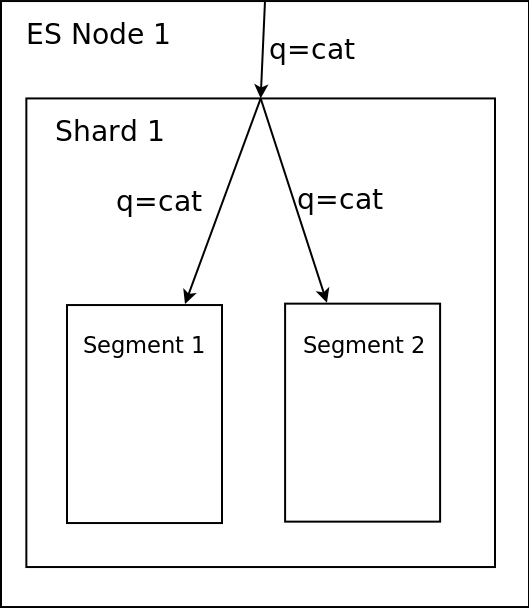
\includegraphics[width=\textwidth,height=7cm,keepaspectratio=true]{search5}
	\end{figure}
\end{frame}
\begin{frame}{Search}
	\begin{figure}
		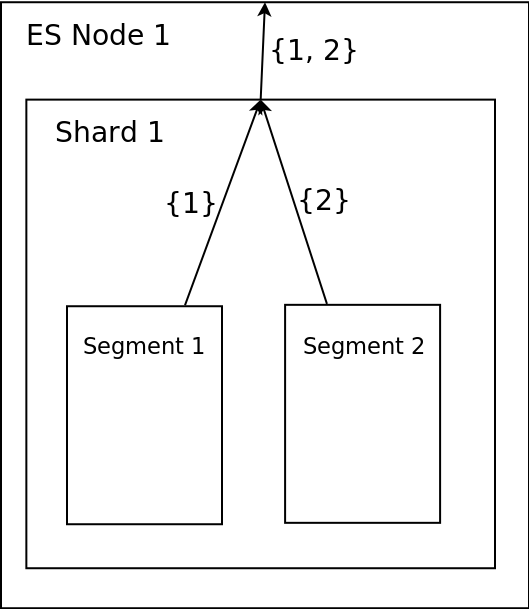
\includegraphics[width=\textwidth,height=7cm,keepaspectratio=true]{search6}
	\end{figure}
\end{frame}
\begin{frame}{Search}
	\begin{figure}
		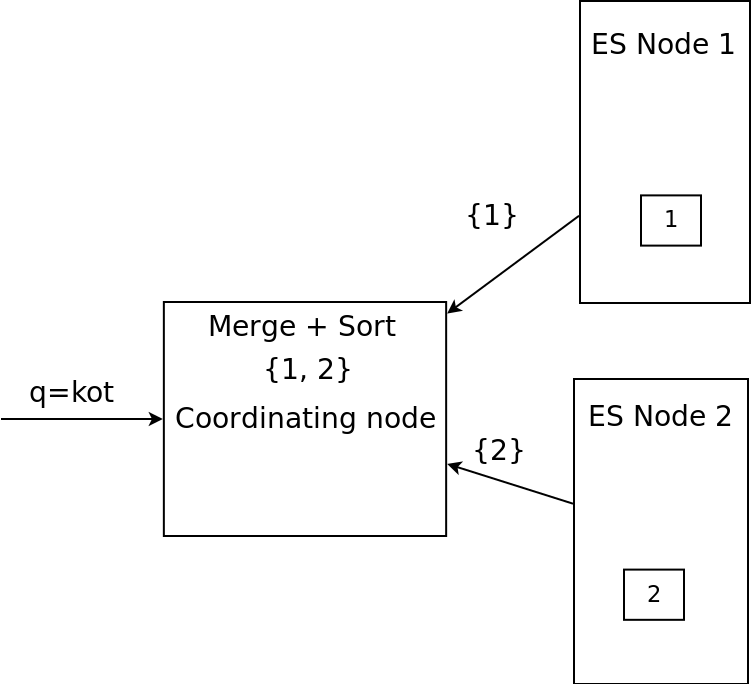
\includegraphics[width=\textwidth,height=7cm,keepaspectratio=true]{search2}
	\end{figure}
\end{frame}
\begin{frame}{Search}
	\begin{figure}
		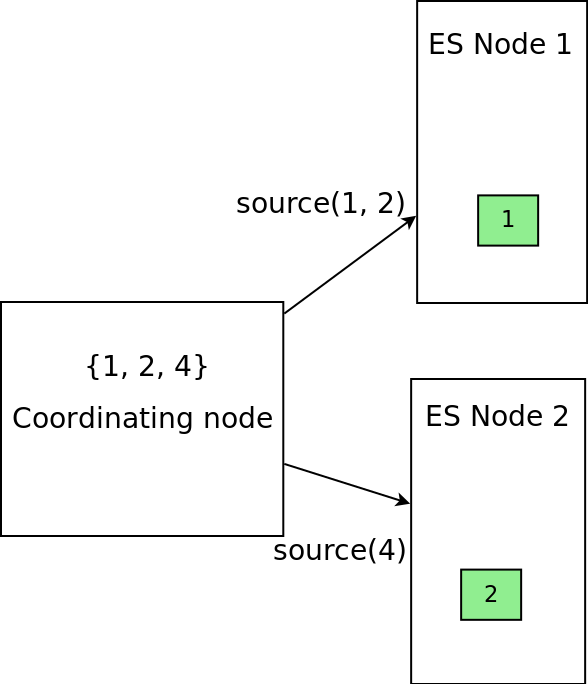
\includegraphics[width=\textwidth,height=7cm,keepaspectratio=true]{search3}
	\end{figure}
\end{frame}
\begin{frame}{Search}
	\begin{figure}
		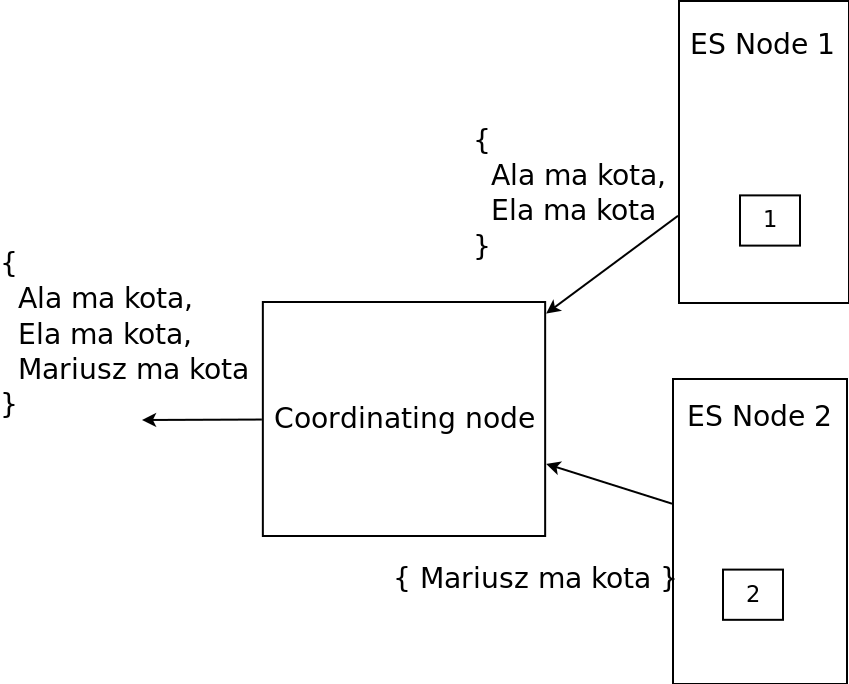
\includegraphics[width=\textwidth,height=7cm,keepaspectratio=true]{search4}
	\end{figure}
\end{frame}
\begin{frame}{Indexing}
	\begin{figure}
		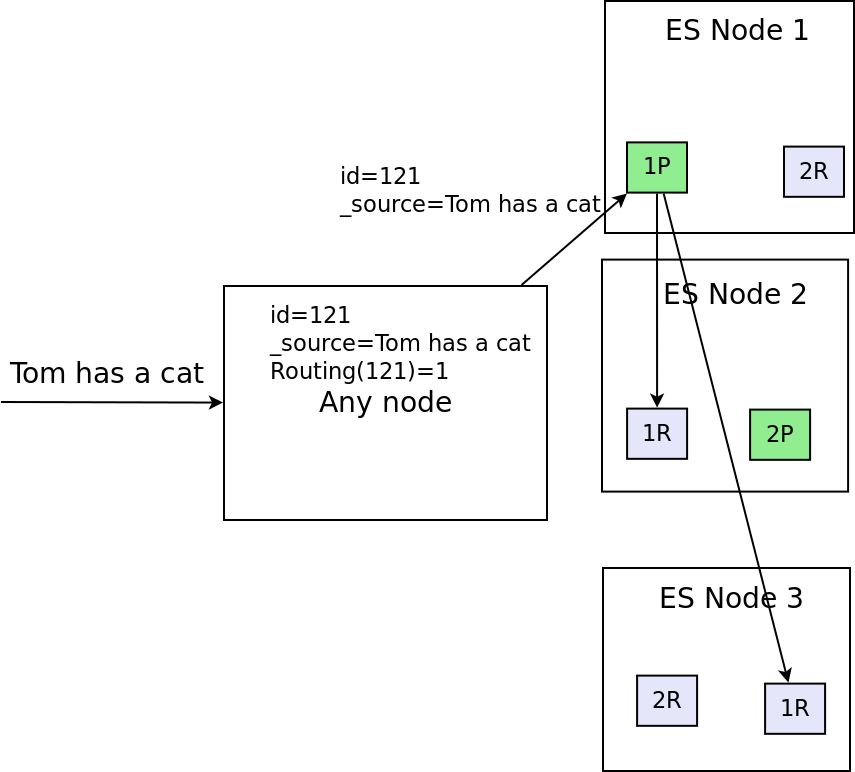
\includegraphics[width=\textwidth,height=7cm,keepaspectratio=true]{indexing}
	\end{figure}
\end{frame}
\begin{frame}{Queries}
	\begin{enumerate}
		\item term
		\item bool
		\item prefix
		\item wildcard
		\item fuzzy
		\item match, match\_all
		\item query\_string
		\item filter vs query
	\end{enumerate}
\end{frame}
\begin{frame}{Analyzers}
	\begin{enumerate}
		\item whitespace
		\item standard
		\item keyword
	\end{enumerate}
\end{frame}{
\begin{frame}{Custom analyzer}
	\begin{enumerate}
		\item char\_filters - removes / changes / adds characters before text goes to tokenizer
		\item tokenizer - splits text into tokens
		\item filters - removes / changes / adds tokens
	\end{enumerate}
\end{frame}{
\begin{frame}{Indexing}
	\begin{figure}
		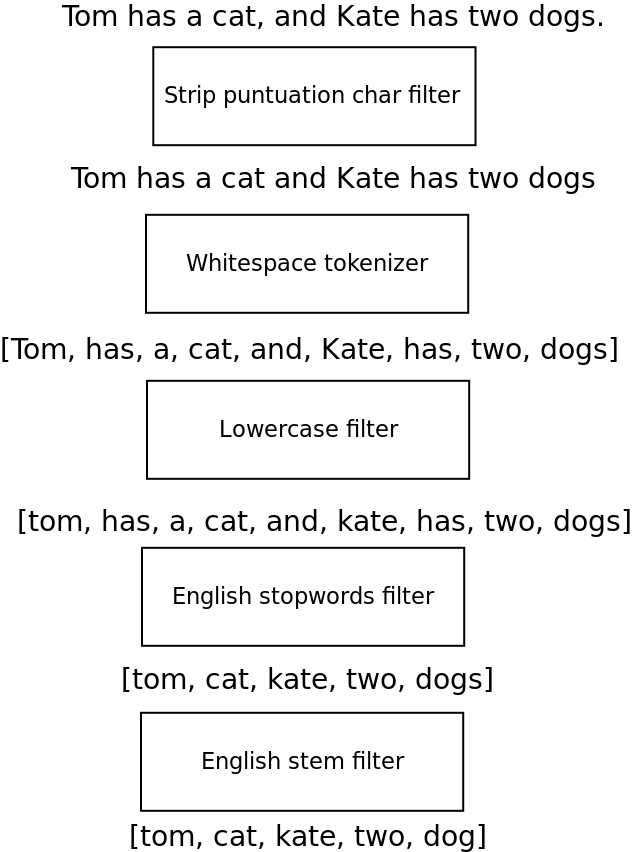
\includegraphics[width=\textwidth,height=7cm,keepaspectratio=true]{analyzer}
	\end{figure}
\end{frame}
\begin{frame}{Scoring}
	\begin{equation*}
	\begin{multlined}
score(q,d) = \\
	queryNorm(q) * coord(q,d) * \\
	\sum(tf(t\ in\  d) *  idf(t)^2 * t.getBoost() *  norm(t,d)) (t\ in\ q)    
	\end{multlined}
	\end{equation*}
\end{frame}
\begin{frame}{Scoring}
	\begin{enumerate}
		\item score(q,d) - the relevance score of document d for query q
		\item queryNorm(q) - query normalization factor
		\item coord(q,d) is the coordination factor (rewards for higher percentage of query terms contained in document)
		\item tf(t in d) - term frequency for term t in document d,
		\item idf(t) - inverse document frequency for term t,
		\item t.getBoost() - boost that has been applied to the query,
		\item norm(t,d) - field-length norm, combined with the index-time field-level boost
	\end{enumerate}
	\begin{center}
		{\tiny (https://www.elastic.co/guide/en/elasticsearch/guide/current/practical-scoring-function.html)}
	\end{center}
\end{frame}
\begin{frame}{Cluster}
	\begin{enumerate}
		\item Master node - keeping, updating, broadcasting state of the cluster (list of nodes, mappings)
		\item Data node - storing data and executing searches on shard
		\item Access node -  forwarding requests to data nodes and merging results
		\item Ingest node - preprocess documents before indexing them
	\end{enumerate}
\end{frame}
\begin{frame}{Leader election}
	\begin{enumerate}
		\item zen discovery
		\item leader election
		\item quorum
	\end{enumerate}
\end{frame}
\begin{frame}{Cluster}
	\begin{figure}
		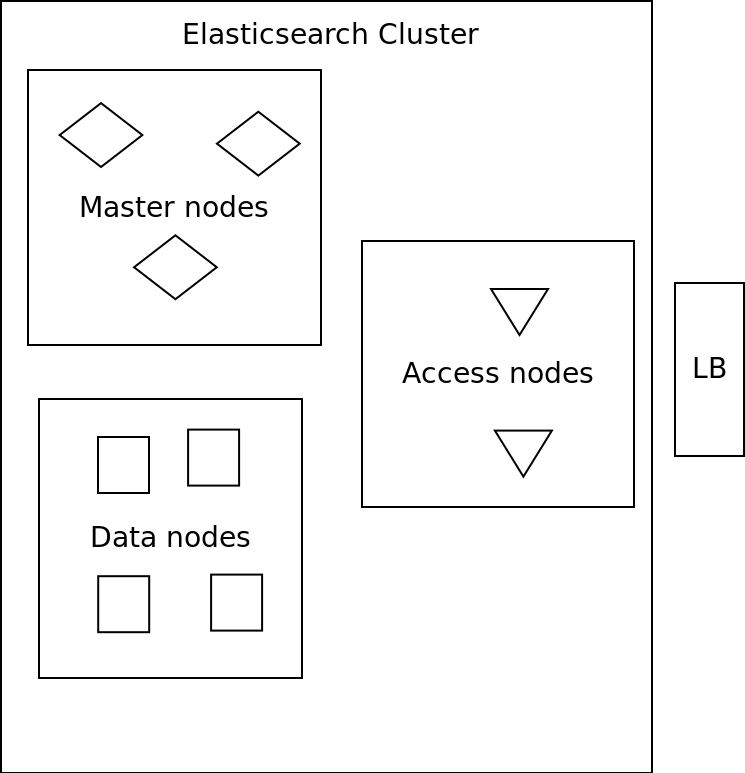
\includegraphics[width=\textwidth,height=7cm,keepaspectratio=true]{cluster}
	\end{figure}
\end{frame}
\section{Questions?}

\end{document}
